\documentclass{article}
% -------- Umlaute korrekt ----------------
\usepackage[latin1, utf8]{inputenc}
\usepackage[ngerman]{babel}
\usepackage{graphicx}
\usepackage{pdfpages}
\usepackage{amsmath}
\usepackage{amssymb}
%-------------------------------------------

% Einrueckung unterbinden nach Absatz
\setlength{\parindent}{0pt}


\DeclareMathSizes{10}{10}{10}{10}
\title{RA -- R\"U Blatt 2}
\author{Christian Bay (lu38wuqi), Tobias Miksch (up83yvev)}
\date{\today}
\begin{document}
\maketitle

\textbf{ICC Version:}
\begin{enumerate}
	\item intelmpi/4.1.3.048-intel
	\item mkl/11.0up05
	\item intel64/13.1up03
\end{enumerate}

\textbf{Emmy Cluster}
\begin{enumerate}
	\item Taktfrequenz: 2.2 GHz
\end{enumerate}

\vspace*{6pt}

\section*{Aufgabe 2}
\begin{tabular}{ c | c | c |}
Single Precision &	SSE			& AVX \\
	\hline
	\#Ups & 159 & 170\\
	\hline
	Cycles & 40 & 42\\
	\hline
	Throughput & 0.25 & 0.23 \\
	\hline
\end{tabular}



\vspace*{10pt}
Erwartete \textbf{Mup/s}:\\
\begin{align*}
	\text{MUPS}_{\text{SSE: }} (0.25*159) * (2.2 * 10^3) = 87450\\
	\text{MUPS}_{\text{AVX: }} (0.23*170) * (2.2 * 10^3) = 86020
\end{align*}
\section*{Aufgabe 3}
\subsection*{b)}

\begin{center}
	\begin{figure}[h]
	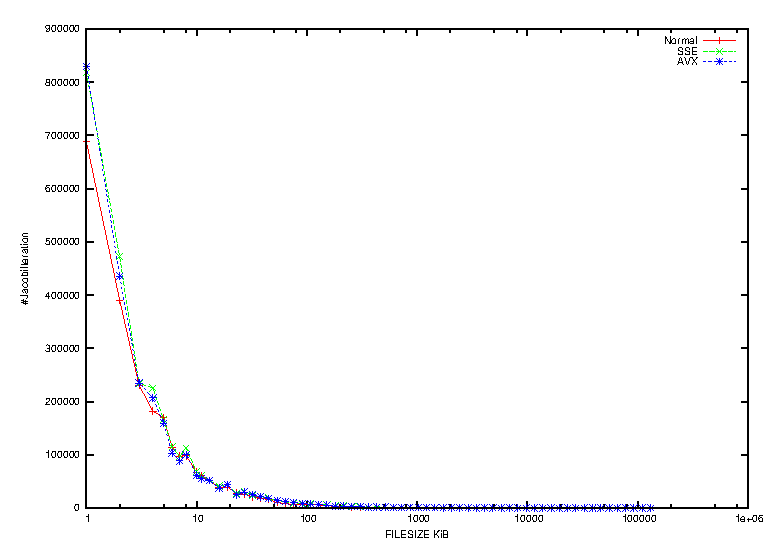
\includegraphics[scale=0.75]{images/float.eps}
		\caption{Plot of with float entries}
	\end{figure}
\end{center}

\begin{center}
	\begin{figure}[h]
	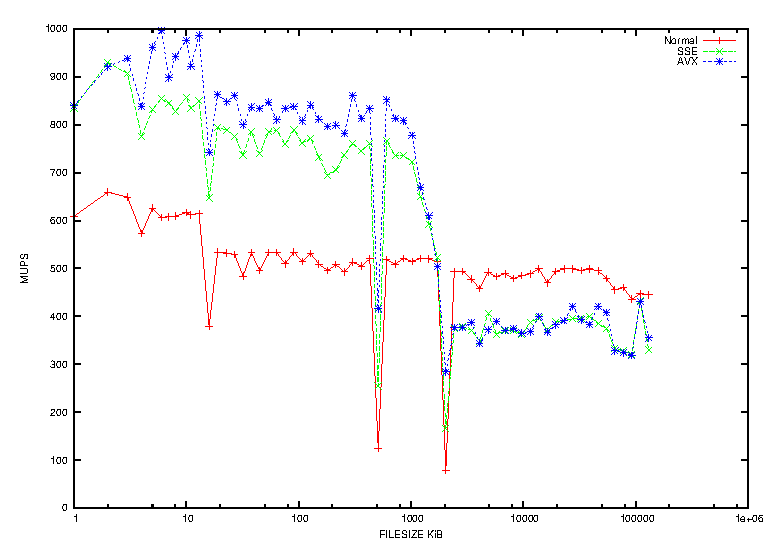
\includegraphics[scale=0.75]{images/double.eps}
		\caption{Plot of with double entries}
	\end{figure}
\end{center}

\end{document}
